\documentclass[border=6pt]{standalone}
\usepackage{amsmath,amssymb}
\usepackage{tikz}
\usetikzlibrary{decorations.pathreplacing,calc,positioning}
% TikZ styles and helpers shared by figures/circuits.tex and figures/circuits_qsvt.tex
\tikzset{
  wire/.style={line width=0.55pt},
  gate/.style={draw,fill=white,minimum height=6.2mm,minimum width=7.5mm,inner sep=1.5pt,font=\small,line width=0.55pt},
  wgate/.style={gate,minimum width=13mm},
  ctrl/.style={circle,fill=black,inner sep=0pt,minimum size=1.9mm},
  octrl/.style={circle,draw,fill=white,inner sep=0pt,minimum size=1.9mm,line width=0.55pt},
  targ/.style={circle,draw,inner sep=0pt,minimum size=3.2mm,line width=0.55pt},
  meter/.style={draw,fill=white,minimum height=6.2mm,minimum width=7.5mm,line width=0.55pt},
  reg/.style={font=\small,anchor=east},
  blk/.style={font=\footnotesize,anchor=north,text=black!65},
  st/.style={font=\footnotesize,anchor=south,text=blue!45!black},
  brace/.style={decorate,decoration={brace,mirror,amplitude=2.2pt},line width=0.4pt,black!60},
  slash/.style={},
}
\newcommand{\slashwire}[3]{% x y label : the /n mark on a multi-qubit wire
  \draw[line width=0.7pt] (#1cm-1.3mm,#2cm-1.6mm) -- (#1cm+1.3mm,#2cm+1.6mm);
  \node[font=\scriptsize,anchor=south west,inner sep=0.4pt] at (#1cm+0.9mm,#2cm+0.9mm) {#3};}
\newcommand{\vsep}[3]{% x ybot ytop : a dashed block boundary
  \draw[dashed,black!45,line width=0.4pt] (#1cm,#2cm) -- (#1cm,#3cm);}


% box spanning wires: x, ytop, ybot, width(cm), label
\newcommand{\mb}[5]{\draw[fill=white,line width=0.55pt] (#1-#4/2,#2+0.31) rectangle (#1+#4/2,#3-0.31); \node[font=\small] at (#1,{(#2+#3)/2}) {#5};}
\newcommand{\gt}[3]{\node[gate] at (#1,#2) {#3};}
\newcommand{\wg}[4]{\node[gate,minimum width=#3] at (#1,#2) {#4};}
\newcommand{\ct}[2]{\node[ctrl] at (#1,#2) {};}
\newcommand{\oc}[2]{\node[octrl] at (#1,#2) {};}
\newcommand{\vl}[3]{\draw[wire] (#1,#2) -- (#1,#3);}
\newcommand{\tg}[2]{\node[targ] at (#1,#2) {}; \draw[wire] (#1,#2-0.16) -- (#1,#2+0.16);}
\newcommand{\meas}[2]{\node[meter] at (#1,#2) {}; \draw[wire] (#1-0.25,#2-0.12) arc (160:20:0.27); \draw[wire,-latex] (#1,#2-0.12) -- (#1+0.2,#2+0.12);}
\newcommand{\wires}[3]{\foreach \y in {#3} {\draw[wire] (#1,\y) -- (#2,\y);}}
\newcommand{\lab}[3]{\node[reg] at (#1,#2) {#3};}
\definecolor{hitp}{RGB}{118,68,160}
\definecolor{classic}{RGB}{90,90,90}
\newcommand{\cbox}[6]{\draw[rounded corners=3pt,fill=black!4,draw=black!45,line width=0.5pt] (#1,#2) rectangle (#3,#4); \node[font=\footnotesize,align=center,text width=#6] at ({(#1+#3)/2},{(#2+#4)/2}) {#5};}
\begin{document}

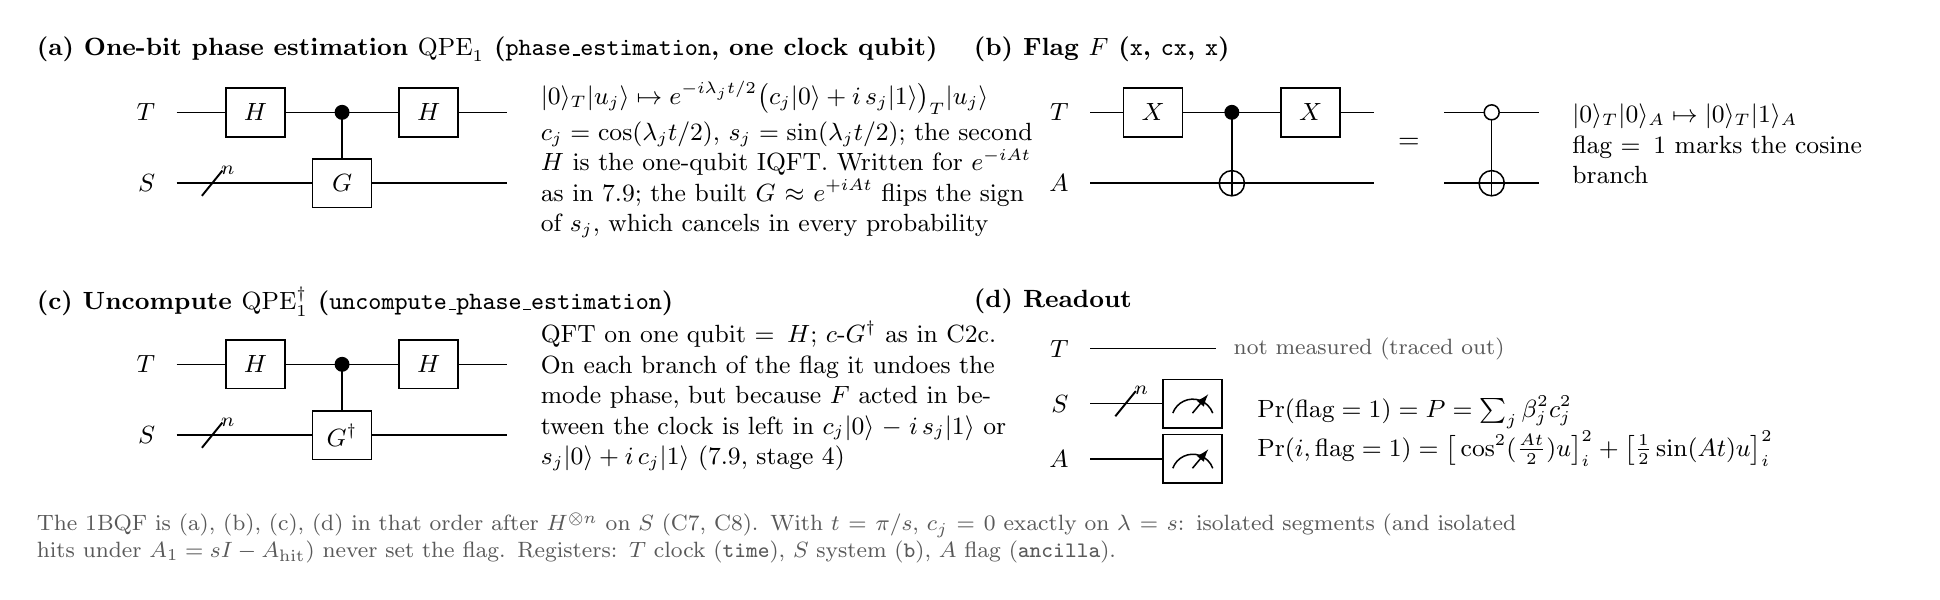
\begin{tikzpicture}[x=1cm,y=1cm]
% (a) QPE_1
\node[anchor=west,font=\small\bfseries] at (-1.9,1.2) {(a) One-bit phase estimation $\mathrm{QPE}_1$ (\texttt{phase\_estimation}, one clock qubit)};
\lab{-0.15}{0.4}{$T$} \lab{-0.15}{-0.5}{$S$}
\wires{0}{4.2}{0.4,-0.5} \slashwire{0.45}{-0.5}{$n$}
\gt{1.0}{0.4}{$H$} \ct{2.1}{0.4} \vl{2.1}{0.4}{-0.5} \gt{2.1}{-0.5}{$G$} \gt{3.2}{0.4}{$H$}
\node[font=\small,anchor=west,text width=6.3cm] at (4.5,-0.2) {$|0\rangle_T|u_j\rangle\mapsto e^{-i\lambda_jt/2}\big(c_j|0\rangle+i\,s_j|1\rangle\big)_T|u_j\rangle$\\[2pt] $c_j=\cos(\lambda_jt/2)$, $s_j=\sin(\lambda_jt/2)$; the second $H$ is the one-qubit IQFT. Written for $e^{-iAt}$ as in 7.9; the built $G\approx e^{+iAt}$ flips the sign of $s_j$, which cancels in every probability};
% (b) flag
\begin{scope}[shift={(11.6,0)}]
\node[anchor=west,font=\small\bfseries] at (-1.6,1.2) {(b) Flag $F$ (\texttt{x}, \texttt{cx}, \texttt{x})};
\lab{-0.15}{0.4}{$T$} \lab{-0.15}{-0.5}{$A$}
\wires{0}{3.6}{0.4,-0.5}
\gt{0.8}{0.4}{$X$} \ct{1.8}{0.4} \vl{1.8}{0.4}{-0.5} \tg{1.8}{-0.5} \gt{2.8}{0.4}{$X$}
\node at (4.05,0) {$=$};
\wires{4.5}{5.7}{0.4,-0.5} \oc{5.1}{0.4} \vl{5.1}{0.32}{-0.5} \tg{5.1}{-0.5}
\node[font=\small,anchor=west,text width=4.2cm] at (6.0,0) {$|0\rangle_T|0\rangle_A\mapsto|0\rangle_T|1\rangle_A$\\ flag $=1$ marks the cosine branch};
\end{scope}
% (c) uncompute
\begin{scope}[shift={(0,-3.2)}]
\node[anchor=west,font=\small\bfseries] at (-1.9,1.2) {(c) Uncompute $\mathrm{QPE}_1^{\dagger}$ (\texttt{uncompute\_phase\_estimation})};
\lab{-0.15}{0.4}{$T$} \lab{-0.15}{-0.5}{$S$}
\wires{0}{4.2}{0.4,-0.5} \slashwire{0.45}{-0.5}{$n$}
\gt{1.0}{0.4}{$H$} \ct{2.1}{0.4} \vl{2.1}{0.4}{-0.5} \gt{2.1}{-0.5}{$G^\dagger$} \gt{3.2}{0.4}{$H$}
\node[font=\small,anchor=west,text width=6.3cm] at (4.5,0) {QFT on one qubit $=H$; $c\text{-}G^\dagger$ as in C2c. On each branch of the flag it undoes the mode phase, but because $F$ acted in between the clock is left in $c_j|0\rangle-i\,s_j|1\rangle$ or $s_j|0\rangle+i\,c_j|1\rangle$ (7.9, stage 4)};
\end{scope}
% (d) measurement
\begin{scope}[shift={(11.6,-3.2)}]
\node[anchor=west,font=\small\bfseries] at (-1.6,1.2) {(d) Readout};
\lab{-0.15}{0.6}{$T$} \lab{-0.15}{-0.1}{$S$} \lab{-0.15}{-0.8}{$A$}
\wires{0}{1.6}{0.6} \wires{0}{1.0}{-0.1,-0.8} \slashwire{0.45}{-0.1}{$n$}
\node[font=\footnotesize,anchor=west,text=black!65] at (1.7,0.6) {not measured (traced out)};
\meas{1.3}{-0.1} \meas{1.3}{-0.8}
\node[font=\small,anchor=west,text width=7.2cm] at (2.0,-0.45) {$\Pr(\text{flag}=1)=P=\sum_j\beta_j^2c_j^2$\\ $\Pr(i,\text{flag}=1)=\big[\cos^2(\tfrac{At}{2})u\big]_i^2+\big[\tfrac12\sin(At)u\big]_i^2$};
\end{scope}
\node[font=\footnotesize,anchor=west,text=black!65,text width=19cm] at (-1.9,-5.0) {The 1BQF is (a), (b), (c), (d) in that order after $H^{\otimes n}$ on $S$ (C7, C8). With $t=\pi/s$, $c_j=0$ exactly on $\lambda=s$: isolated segments (and isolated hits under $A_1=sI-A_{\rm hit}$) never set the flag. Registers: $T$ clock (\texttt{time}), $S$ system (\texttt{b}), $A$ flag (\texttt{ancilla}).};
\end{tikzpicture}
\end{document}
